\chapter{Testing} % Detailed descriptions of every test case are definitely not what is required here. What is important is to show that you adopted a sensible strategy that was, in principle, capable of testing the system adequately even if you did not have the time to test the system fully.Have you tested your system on �real users�? For example, if your system is supposed to solve a problem for a business, then it would be appropriate to present your approach to involve the users in the testing process and to record the results that you obtained. Depending on the level of detail, it is likely that you would put any detailed results in an appendix.The following sections indicate some areas you might include. Other sections may be more appropriate to your project. 

SmartResolution is an open-source platform being marketed to those wanting to provide ODR services, and as such it is very important that the platform itself is thoroughly tested. Clients need to have confidence that the core platform works as it should, and module developers need to have confidence that the underlying system is robust enough to support their module. For these reasons, the core platform implementation was done alongside unit and integration tests.

In an ideal world, the same principles would be applied to the Maritime Collision module and to the SmartResolution Marketplace. However, developing the core platform in a test-driven way turned out to be quite a slow, methodical process - read more in the `Evaluation' section - and I felt that doing the same for the lesser two components was a luxury I could not afford with an impeding deadline. Therefore, this section is mostly concerned with testing the core SmartResolution software.

As previously mentioned, the project was developed in an agile way from the implementation onwards. As such, the principles of business-driven development (BDD), test-driven development (TDD) and continuous integration (CI) were applied throughout the implementation.

\section{Unit Testing}

Almost every class in the system has an associated unit test. This does not apply to library classes, such as those provided by F3, since the responsibility for testing these lies with the third party.

The nature of unit tests should be that they are loaded into memory and are very quick to run. [REF] ``Unit tests focus just on the class or method at hand. They run entirely in memory, which makes them very fast. Depending on your platform, your testing tool should be able to run at least 100 unit tests per second." % http://www.jamesshore.com/Agile-Book/test_driven_development.html

This makes refactoring less of a headache, since the developer can refactor their code and several times a minute can verify that everything still works as it should.

In that sense, some (though not all) of the unit tests in SmartResolution are not `true' unit tests, as they rely on the database connection. According to Michael Feathers [REF], ``A test is not a unit test if: % http://www.artima.com/weblogs/viewpost.jsp?thread=126923

It talks to the database
It communicates across the network
It touches the file system
It can't run at the same time as any of your other unit tests
You have to do special things to your environment (such as editing config files) to run it.''

At this stage, it is more important to have a complete set of tests than a test suite than can be run quickly. That said, speed is important to the developer workflow, and was something that I concentrated on improving towards the end of the project.

\subsection{Database transaction threads}

Between test suites, SmartResolution runs the `clear database' command to revert the database to a known constant: an untainted database filled with predefined fixture data. This reverses any changes that may have been made to the database when running the previous test suite, e.g. a test that enables round-table communication in a dispute would be reverted to the state of the communication of the dispute in the fixture data.

This is a useful technique in ensuring that test suites don't corrupt one another's results and that each suite works with the same set of data. However, it is slow, since the process requires removing the test SQLite database, re-creating it and then re-populating it through PHP's \lstinline{shell_exec} command. This takes around a second on a reasonably powerful machine, so becomes a problem if the script is called dozens or even hundreds of times.

I made a conscious effort to keep these resets to a minimum, but a problem I faced early on in my unit tests was the following error message:

``PDOException: There is already an active transaction!"

The exception refers to database transactions. Often, we want to accomplish several things in one `transaction', for example, debiting one person's account and crediting the other person's account. If the debiting of the first person's account fails - for example, if doing so would make their account balance a negative value - then we don't want the other person's account to be credited. Both queries must happen, or neither must happen.

In PDO (PHP Data Objects), and in F3's wrapper for PDO, we are able to define the start and end points of a transaction. We would say ``begin transaction", debit the first account, credit the second account, and then say ``commit transaction". If either query in the transaction failed, then neither would be applied.

The exception message mentioned earlier refers to a situation whereby a transaction was begun, perhaps some queries were queued for the transaction, and then there was another request to begin a transaction. Somewhere in SmartResolution, a transaction was not being committed or rolled back.

This wasn't too much of an issue. As a quick fix, I was able to run the `clear database' command between any unit tests that raised this exception, as clearing the database would naturally clear any outstanding transactions. I didn't feel that this was too much of an issue, as the test and production environments are very different. The exception was being raised because hundreds of transactions were happening when running the unit tests, as all tests are hooking into the same database connection. In the production environment this would not happen as transactions are only applied for the action the user wants to perform, not for testing the entire system at once.

For several weeks, I was happy with this solution, but it did mean that my tests were quite slow to run. You can see in a Travis build around that time [REF] that it took almost a minute to run 90 unit tests. % https://travis-ci.org/ChrisBAshton/smartresolution/builds/58603809

Eventually, I decided to spend some time investigating the issue. I deduced that the transaction was not being committed because an exception was being raised before it could be committed. This was normal, since my unit tests were supposed to be testing the exceptions.

What I did not realise was that transactions were not being automatically rolled back when an exception was raised - it was something that needed to be handled manually in each exception. This seemed laborious, error-prone and messy.

Instead, I defined a custom exception function [REF] which throws an exception, but also rolls back any existing transactions. Now, unit tests could be run without clearing the database in between each test. % https://github.com/ChrisBAshton/smartresolution/blob/b33f30064048d2dc6c84d72736dcdacb02d293b9/webapp/core/model/Utils.php#L14-L25

\begin{lstlisting}
    public function throwException($message) {
        try {
            Database::instance()->rollback();
        } catch (Exception $PDOException) {
            // do nothing - we only wanted to roll back the transaction if one existed.
            // since one doesn't exist, there's nothing to roll back. Let's just continue and
            // throw the Exception we wanted to throw in the first place.
        }
        throw new Exception($message);
    }
\end{lstlisting}

This led to big improvements in test speed: at this stage, I could now run 112 unit tests in just 34 seconds [REF]. This is 3.29 unit tests per second (UTPS), compared with 1.58 UTPS before the optimisation. % https://travis-ci.org/ChrisBAshton/smartresolution/builds/58932345

I still needed to clear the database between each test \emph{suite}, as the tests would still alter the state of the database. But now, by and large, most of the tests \emph{within} those suites do not need to run on a new database connection.

\subsection{Refactoring to pure unit tests}

Earlier I described how `pure' unit tests should not query a database. An unfortunate consequence of the implementation of my code is that database querying is essential to unit test my classes, as they are populated by an ID representing a row in the database, rather than populated with an array of data which may or may not have come from a database.

This is an oversight that was impossible to reverse in the last few weeks of the project, as this type of class design was too tightly embedded throughout the entire system. However, if I had unlimited time, this is something I would refactor, for a purer design and to make writing and maintaining tests easier.

Currently, the classes (such as Message) are passed an ID to the constructor. Inside the constructor, a function call is made to a data wrapper class which contains the business logic for retrieving the class-specific data (such as message content, author ID, etc) from the given ID. The returned array is then used to populate the model.

This decouples the model from the database - all SQL queries are encapsulated in the intermediary database querying objects - however, in hindsight, the reverse should have been applied. The SmartResolution core platform's controllers and views should have referred to the database querying objects directly; these would internally refer to the `pure' models, which were instantiated with array data rather than a database ID.

Reversing the entire topology of the framework would be a significant feat of refactoring, worth doing but too high-risk to attempt so close to the project deadline.

\section{Functional Testing}

Every feature of the SmartResolution core software is defined as a Cucumber feature, associated with step definitions, to make each feature executable and automatically verify that the system is working as expected.

As a reminder, the full list of tested features is outlined in appendix~\ref{appendix:requirements}, and the justification for the choice of Ruby and Cucumber as the BDD framework is in appendix~\ref{appendix:bdd}.

Unit tests are tightly coupled to the specific implementation of the code, making refactoring difficult if you wish to move methods, rename classes and the like. Cucumber features, on the other hand, can be defined completely separately from the software itself and are highly valuable since they still test the expected end-to-end functionality of the system as a whole. This makes refactoring the codebase a much less painful process. A necessary principle of unit tests is that the tests will break if the code changes its external API.

\subsection{Using the test database for Cucumber tests}

Cucumber regression tests are end-to-end and use a headless browser to emulate the browser environment, clicking buttons and filling in forms, then querying the state of the HTML to validate that an element of functionality worked as expected.

To accomplish this, the driver (in our case, Poltergeist [REF]) needs to be able to access the server. However, our tests rely on the database having certain fixture-data. Moreover, our tests will be making persistent changes to the database - so it's essential that the tests use a test database, rather than the production database.

As far as the server is concerned, Poltergeist sends a HTTP request, just like any normal user on a normal browser. Poltergeist needed to be able to send a flag, to explicitly inform the application that the request is coming from a test suite and, thus, should be using a test database.

Poltergeist allows you to override the HTTP headers sent with each request, so my Cucumber tests modify the User-Agent property to be either `Poltergeist' or `Poltergeist--clear'. Both headers inform the application that it should use the test database, but the latter provides an additional instruction that the database should be cleared and re-populated with test data before processing the request. This is demonstrated in figure~\ref{uml:headers}.

\begin{figure}[h!]
  \centering
    \ifimages
    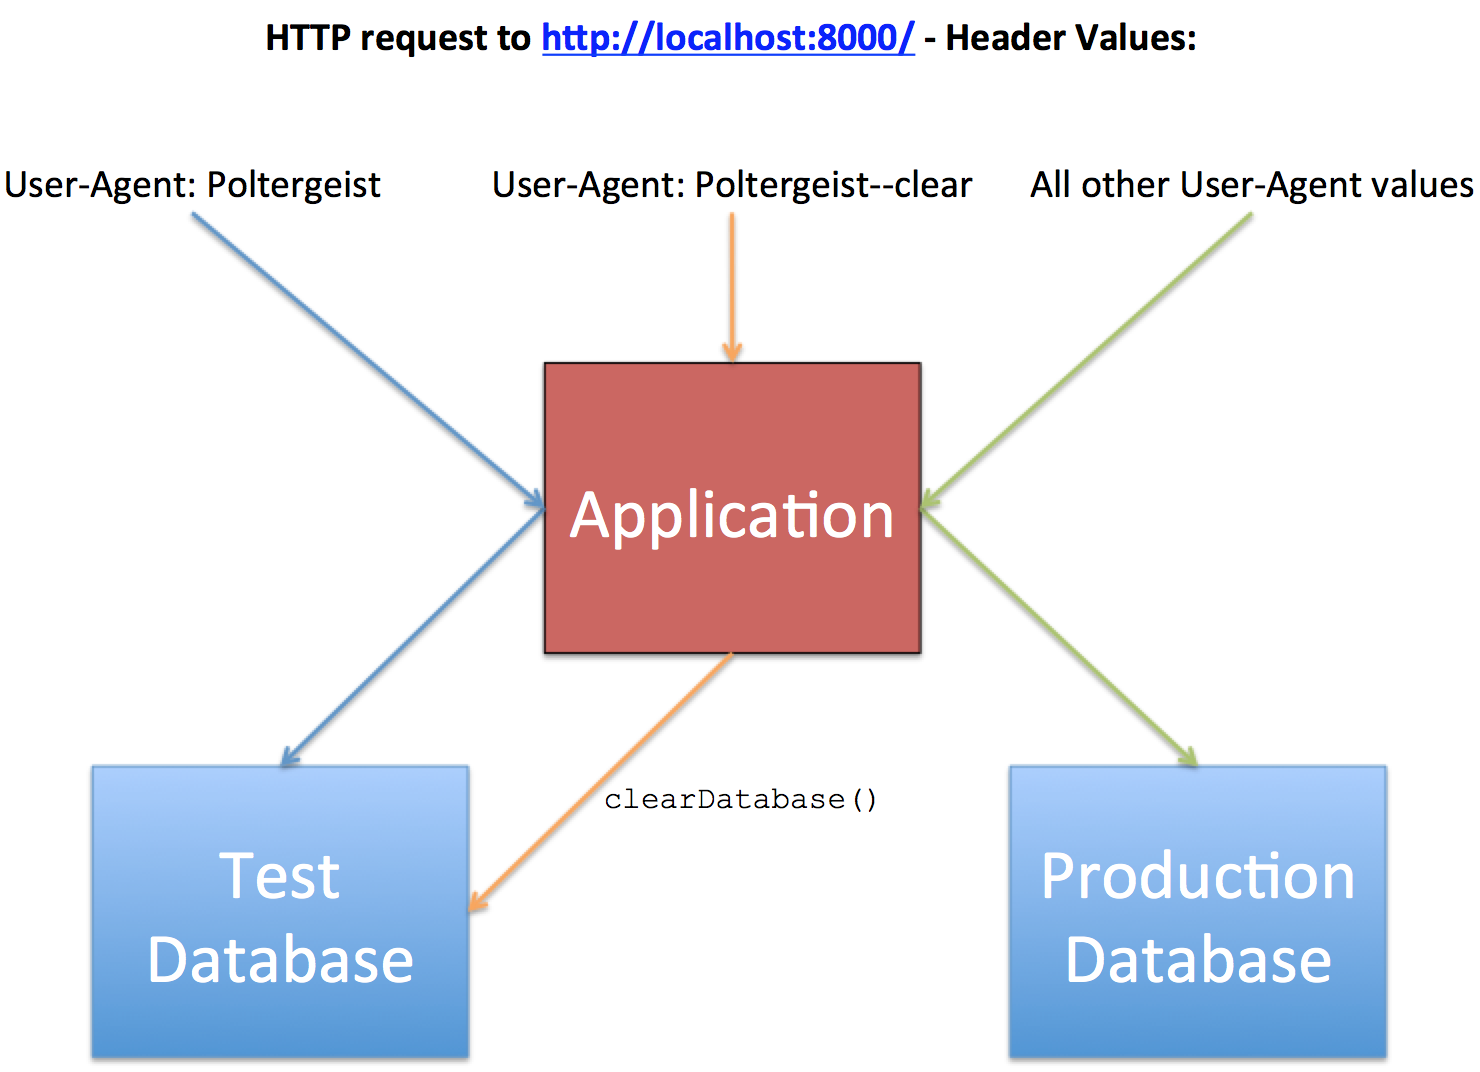
\includegraphics[width=\textwidth]{headers}
    \fi
  \caption{Visualisation of how SmartResolution determines which database to use depending on the received HTTP headers}
  \label{uml:headers}
\end{figure}

There's nothing stopping the end-user changing the headers that they send, so they too could access SmartResolution and interact with the test environment rather than the production environment. Ultimately, this is completely harmless. The test database is cleaned every time the test suite is run, so they would not even be able to sabotage the tests. This is a tried and tested technique, and has been adopted by companies including the BBC [REF].

\subsection{Integration tests structure}

@TODO - explain the common/helper classes in step definitions.

Also

@TODO - explain and discuss the tradeoff between descriptive and overly-bogged-down cucumber features. (maybe copy from Ruby assignment)

\section{Continuous Integration}

Travis Continuous Integration [REF] ran my tests on every pushed commit or pull request, automatically running all unit and functional tests and notifying me via email if anything broke.

@TODO - discuss how difficult it was to get PHP server running

\section{User Testing}

Demo with Konstantina